\hypertarget{pillow}{%
\subsection{Pillow}\label{pillow}}

PIL:Python Imaging Library,已经是 Python
平台事实上的图像处理标准库了。PIL 功能非常强大,但 API 却非常简单易用。

由于 PIL 仅支持到 Python 2.7,加上年久失修,于是一群志愿者在 PIL
的基础上创建了兼容的版本,名字叫
\href{https://github.com/python-pillow/Pillow}{Pillow},支持最新 Python
3.x,又加入了许多新特性,因此,我们可以直接安装使用 Pillow。

\hypertarget{ux5b89ux88c5-pillow}{%
\subsubsection{安装 Pillow}\label{ux5b89ux88c5-pillow}}

如果安装了 Anaconda,Pillow 就已经可用了。否则,需要在命令行下通过 pip
安装:

\begin{pythoncode}
$ pip install pillow
\end{pythoncode}

如果遇到\texttt{Permission\ denied}安装失败,请加上\texttt{sudo}重试。

\hypertarget{ux64cdux4f5cux56feux50cf}{%
\subsubsection{操作图像}\label{ux64cdux4f5cux56feux50cf}}

来看看最常见的图像缩放操作,只需三四行代码:

\begin{pythoncode}
from PIL import Image
im = Image.open('test.jpg')

w, h = im.size
print('Original image size: %sx%s' % (w, h))

im.thumbnail((w
print('Resize image to: %sx%s' % (w

im.save('thumbnail.jpg', 'jpeg')
\end{pythoncode}

其他功能如切片、旋转、滤镜、输出文字、调色板等一应俱全。

比如,模糊效果也只需几行代码:

\begin{pythoncode}
from PIL import Image, ImageFilter
im = Image.open('test.jpg')

im2 = im.filter(ImageFilter.BLUR)
im2.save('blur.jpg', 'jpeg')
\end{pythoncode}

效果如下:

 
 \begin{figure}[htp]
	\centering
	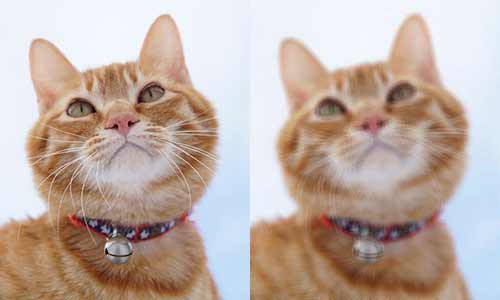
\includegraphics[width=0.6\linewidth]{fig/966760155050624.png}
\end{figure}


PIL
的\texttt{ImageDraw}提供了一系列绘图方法,让我们可以直接绘图。比如要生成字母验证码图片:

\begin{pythoncode}
from PIL import Image, ImageDraw, ImageFont, ImageFilter

import random
def rndChar():
    return chr(random.randint(65, 90))
def rndColor():
    return (random.randint(64, 255), random.randint(64, 255), random.randint(64, 255))
def rndColor2():
    return (random.randint(32, 127), random.randint(32, 127), random.randint(32, 127))
width = 60 * 4
height = 60
image = Image.new('RGB', (width, height), (255, 255, 255))

font = ImageFont.truetype('Arial.ttf', 36)

draw = ImageDraw.Draw(image)

for x in range(width):
    for y in range(height):
        draw.point((x, y), fill=rndColor())

for t in range(4):
    draw.text((60 * t + 10, 10), rndChar(), font=font, fill=rndColor2())

image = image.filter(ImageFilter.BLUR)
image.save('code.jpg', 'jpeg')
\end{pythoncode}

我们用随机颜色填充背景,再画上文字,最后对图像进行模糊,得到验证码图片如下:

 
 \begin{figure}[htp]
	\centering
	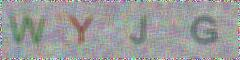
\includegraphics[width=0.6\linewidth]{fig/966760380198752.png}
\end{figure}


如果运行的时候报错:

\begin{pythoncode}
IOError: cannot open resource
\end{pythoncode}

这是因为 PIL
无法定位到字体文件的位置,可以根据操作系统提供绝对路径,比如:

\begin{pythoncode}
'/Library/Fonts/Arial.ttf'
\end{pythoncode}

要详细了解 PIL 的强大功能,请请参考 Pillow 官方文档:

\url{https://pillow.readthedocs.org/}

\hypertarget{ux5c0fux7ed3}{%
\subsubsection{小结}\label{ux5c0fux7ed3}}

PIL 提供了操作图像的强大功能,可以通过简单的代码完成复杂的图像处理。

\hypertarget{ux53c2ux8003ux6e90ux7801}{%
\subsubsection{参考源码}\label{ux53c2ux8003ux6e90ux7801}}

https://github.com/michaelliao/learn-python3/blob/master/samples/packages/pil/use\_pil\_resize.py

https://github.com/michaelliao/learn-python3/blob/master/samples/packages/pil/use\_pil\_blur.py

https://github.com/michaelliao/learn-python3/blob/master/samples/packages/pil/use\_pil\_draw.py

